\documentclass[11pt]{beamer}
% \usetheme{Boadilla}
  \usetheme{default}


% acronyms for text or math mode
\newcommand {\ccast} {\mbox{\small CCAST}}
\newcommand {\cris} {\mbox{\small CrIS}}

\newcommand {\airs} {\mbox{\small AIRS}}
\newcommand {\iasi} {\mbox{\small IASI}}
\newcommand {\idps} {\mbox{\small IDPS}}
\newcommand {\nasa} {\mbox{\small NASA}}
\newcommand {\noaa} {\mbox{\small NOAA}}
\newcommand {\nstar} {\mbox{\small STAR}}
\newcommand {\umbc} {\mbox{\small UMBC}}
\newcommand {\uw}   {\mbox{\small UW}}

\newcommand {\fft}  {\mbox{\small FFT}}
\newcommand {\ifft} {\mbox{\small IFFT}}
\newcommand {\fir}  {\mbox{\small FIR}}
\newcommand {\fov}  {\mbox{\small FOV}}
\newcommand {\for}  {\mbox{\small FOR}}
\newcommand {\ict}  {\mbox{\small ICT}}
\newcommand {\ils}  {\mbox{\small ILS}}
\newcommand {\igm}  {\mbox{\small IGM}}
\newcommand {\opd}  {\mbox{\small OPD}}
\newcommand {\rms}  {\mbox{\small RMS}}
\newcommand {\zpd}  {\mbox{\small ZPD}}
\newcommand {\ppm}  {\mbox{\small PPM}}
\newcommand {\srf}  {\mbox{\small SRF}}
\newcommand {\sdr}  {\mbox{\small SDR}}

\newcommand {\ES} {\mbox{\small ES}}
\newcommand {\SP} {\mbox{\small SP}}
\newcommand {\IT} {\mbox{\small IT}}
\newcommand {\SA} {\mbox{\small SA}}

\newcommand {\ET} {\mbox{\small ET}}
\newcommand {\FT} {\mbox{\small FT}}

% abbreviations, mainly for math mode
\newcommand {\real} {\mbox{real}}
\newcommand {\imag} {\mbox{imag}}
\newcommand {\atan} {\mbox{atan}}
\newcommand {\obs}  {\mbox{obs}}
\newcommand {\calc} {\mbox{calc}}
\newcommand {\sinc} {\mbox{sinc}}
\newcommand {\psinc} {\mbox{psinc}}
\newcommand {\std} {\mbox{std}}

% symbols, for math mode only
\newcommand {\wnum} {\mbox{cm$^{-1}$}}
\newcommand {\lmax} {L_{\mbox{\tiny max}}}
\newcommand {\vmax} {V_{\mbox{\tiny max}}}

\newcommand {\tauobs} {\tau_{\mbox{\tiny obs}}}
\newcommand {\taucal} {\tau_{\mbox{\tiny calc}}}
\newcommand {\Vdc}  {V_{\mbox{\tiny DC}}}

\newcommand {\rIT} {r_{\mbox{\tiny\textsc{ict}}}}
\newcommand {\rES} {r_{\mbox{\tiny\textsc{es}}}}
\newcommand {\robs} {r_{\mbox{\tiny obs}}}

\newcommand {\rITobs} {r_{\mbox{\tiny\textsc{ict}}}^{\mbox{\tiny obs}}}
\newcommand {\rITcal} {r_{\mbox{\tiny\textsc{ict}}}^{\mbox{\tiny cal}}}

\newcommand {\ITmean} {\langle\mbox{\small IT}\rangle}
\newcommand {\SPmean} {\langle\mbox{\small SP}\rangle}


\title{CrIS Nonlinearity Comparisons}
\author{H.~E.~Motteler and L.~L.~Strow}
\institute{
  UMBC Atmospheric Spectroscopy Lab \\
  Joint Center for Earth Systems Technology \\
}
\date{\today}
\begin{document}

%----------- slide --------------------------------------------------%
\begin{frame}[plain]
\titlepage
\end{frame}
%----------- slide --------------------------------------------------%
\begin{frame}
\frametitle{overview}

Small nonlinearities in the \cris\ detector response can be corrected
in ground-segment processing.  We

\begin{itemize}
  \item briefly describe the \ccast\ nonlinearity correction

  \item describe our tests for variation of \fov\ response

  \item compare \ccast\ and \idps\ \fov\ response

  \item look at the effect of adjusting the $a_2$ weights

  \item test the nonlinearity correction in high res mode
\end{itemize}

Our initial motivation for looking into this was to get the
nonlinearity correction working for the \cris\ high res mode

\end{frame}
%----------- slide --------------------------------------------------%
\begin{frame}
\frametitle{ccast nonlinearity} 

\begin{itemize}
  \item the ccast nonlinearity correction follows the \cris\ ATBD with
    the UW form of the correction factor, $1 + 2a_2\Vdc$

  \item count spectra are divided by the numeric filter at the
    sensor grid, in the DC level integral

  \item the numeric filter is taken from time-domain weights, and
    the frequency domain representation needs to be normalized to
    match the filters used for the original $a_2$ fitting

  \item our initial problems with the new filters were resolved with
    this normalization

  \item the time-domain representation of the filter allows the same
    code to work for both regular and high resolution modes
\end{itemize}

\end{frame}
%----------- slide --------------------------------------------------%
\begin{frame}
\frametitle{LW numeric filter}

\begin{center}
  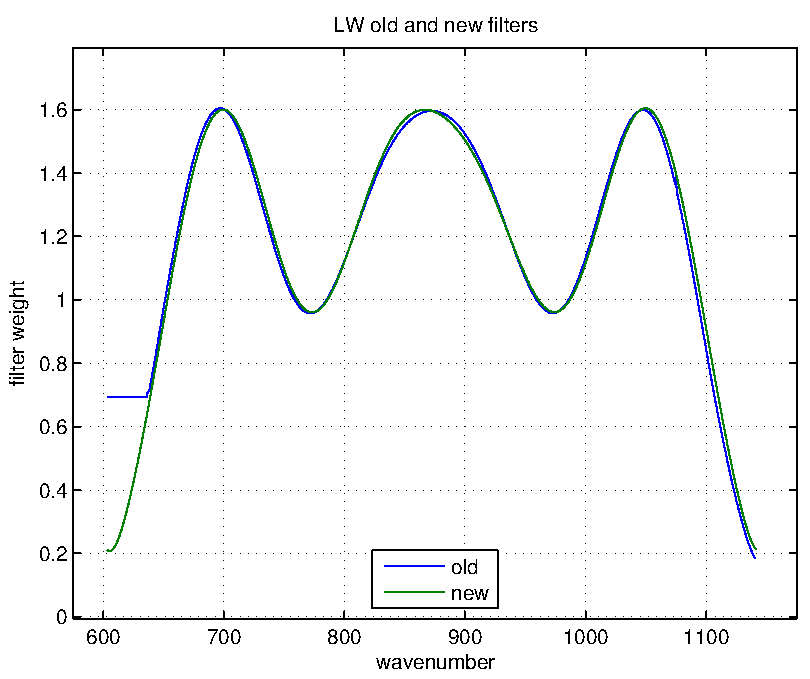
\includegraphics[scale=0.5]{FIR_filter_LW.pdf}
\end{center}

The old (c. 2008) and latest LW numeric filters, with the new filter
normalized to match the old

\end{frame}
%----------- slide --------------------------------------------------%
\begin{frame}
\frametitle{MW numeric filter}

\begin{center}
  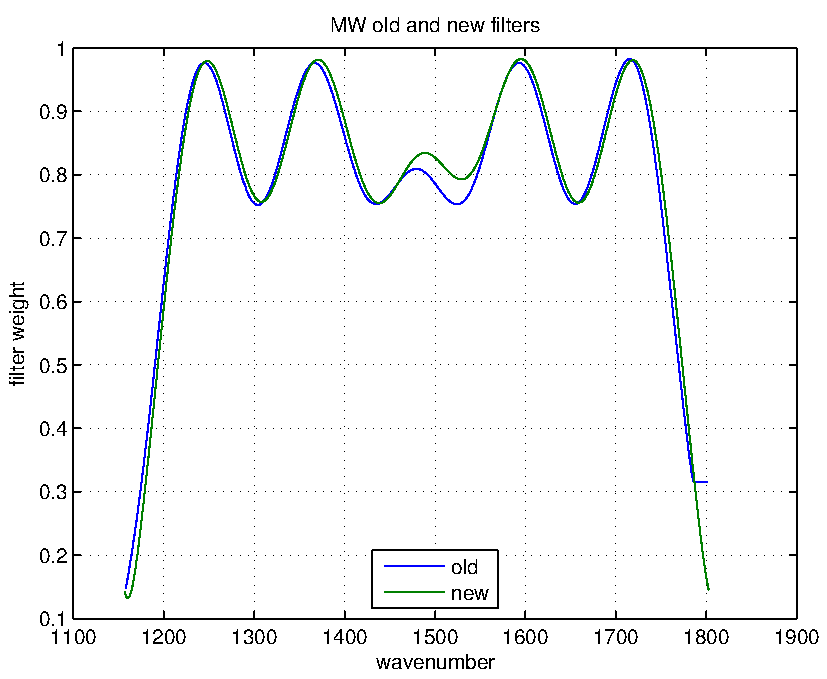
\includegraphics[scale=0.5]{FIR_filter_MW.pdf}
\end{center}

The old and latest MW numeric filters, with the new filter
normalized to match the old

\end{frame}
%----------- slide --------------------------------------------------%
\begin{frame}
\frametitle{SW numeric filter}

\begin{center}
  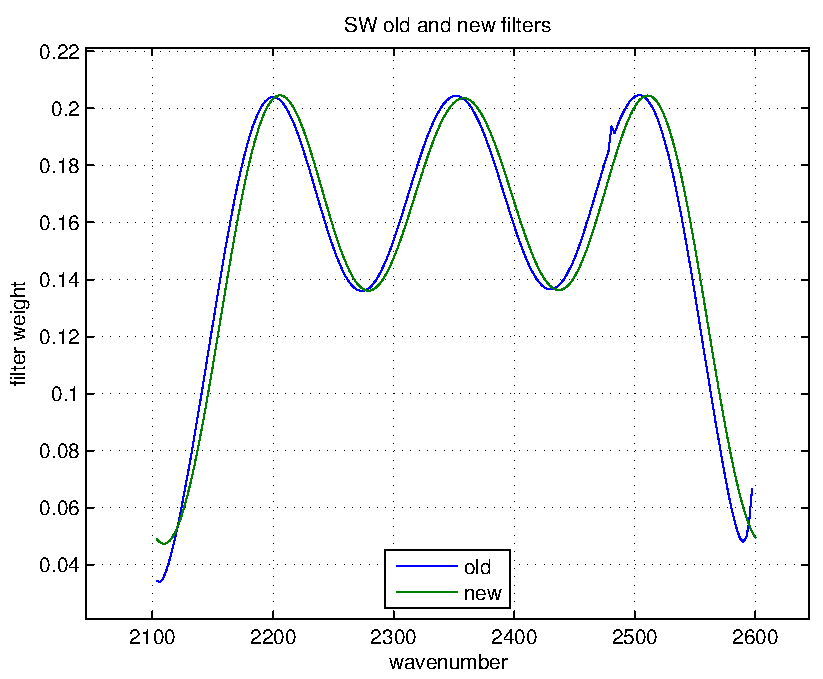
\includegraphics[scale=0.5]{FIR_filter_SW.pdf}
\end{center}

The old and latest SW numeric filters, with the new filter
normalized to match the old

\end{frame}
%----------- slide --------------------------------------------------%
\begin{frame}
\frametitle{test design}

\begin{itemize}
  \item take the average of each FOV over the sample period for FOR
    15 and 16 ascending, and compare these with the average for FOV
    5

  \item to the extent that different FOV views dissappear in the
    averages, this can reveal differences in detector response

  \item the averages are over approximately 10,000 obs per day

  \item we look at sample periods 1-3 Mar 2014, 5-18 Mar 2014,
    and the 27-28 Aug 2013 high resolution test
    
  \item for some tests the ccast processing was rerun with modified
    $a_2$ values
\end{itemize}

These initial tests are comparisons with FOV 5 rather than the most
linear FOV to help sort out geometric or other variations in FOV
response from nonlinearity.

\end{frame}
%----------- slide --------------------------------------------------%
\begin{frame}
\frametitle{ccast LW 2-week test}

\begin{center}
  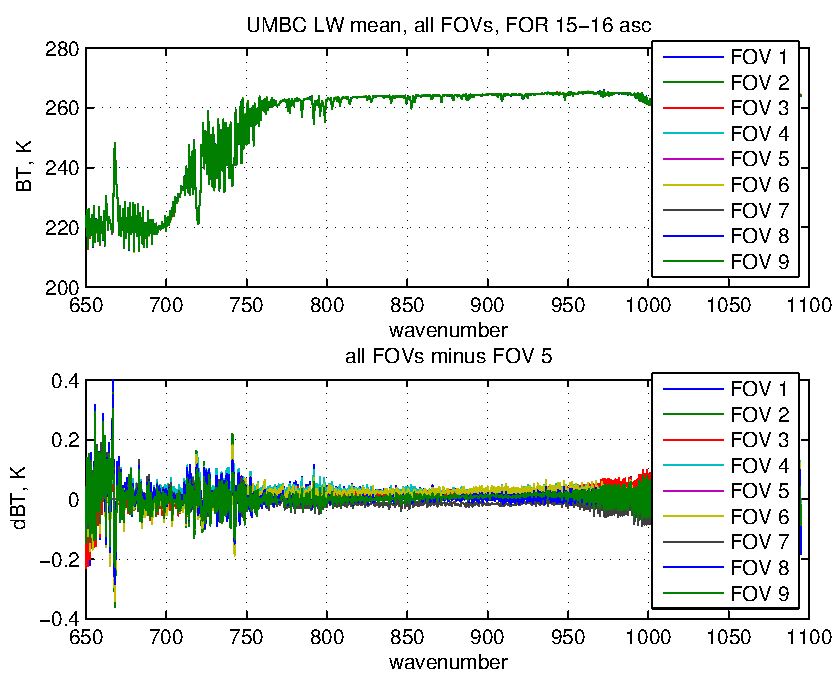
\includegraphics[scale=0.6]{umbc_LW_avg_5-18_Mar.pdf}
\end{center}

\ccast\ LW mean for all FOVs, and for all FOVs minus FOV 5

\end{frame}
%----------- slide --------------------------------------------------%
\begin{frame}
\frametitle{ccast LW 2-week test}

\begin{center}
  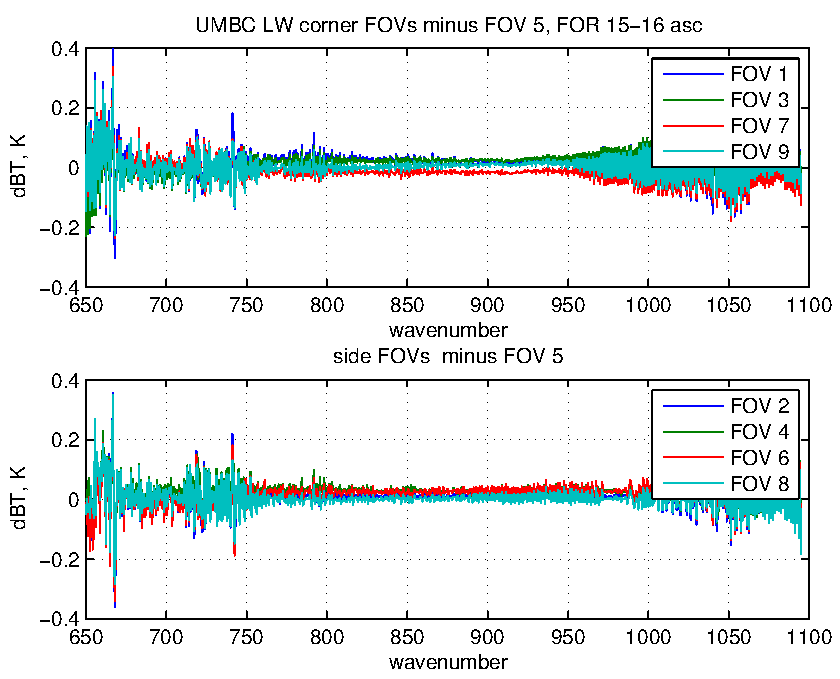
\includegraphics[scale=0.6]{umbc_LW_dif_5-18_Mar.pdf}
\end{center}

\ccast\ LW corner and side FOVs broken out separately

\end{frame}
%----------- slide --------------------------------------------------%
\begin{frame}
\frametitle{IDPS LW 2-week test}

\begin{center}
  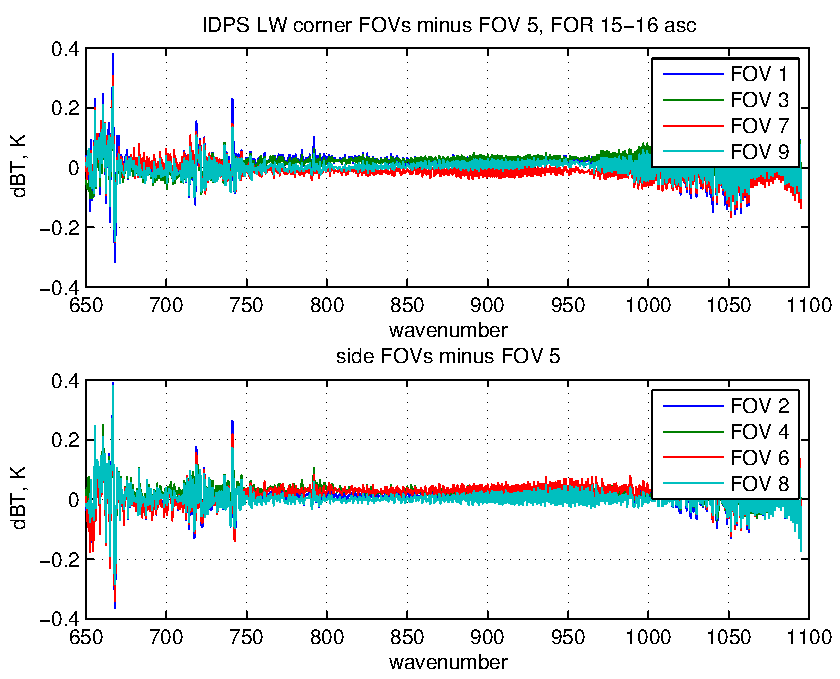
\includegraphics[scale=0.6]{idps_LW_dif_5-18_Mar.pdf}
\end{center}

\idps\ LW corner and side FOVs broken out separately

\end{frame}
%----------- slide --------------------------------------------------%
\begin{frame}
\frametitle{ccast MW 2-week test}

\begin{center}
  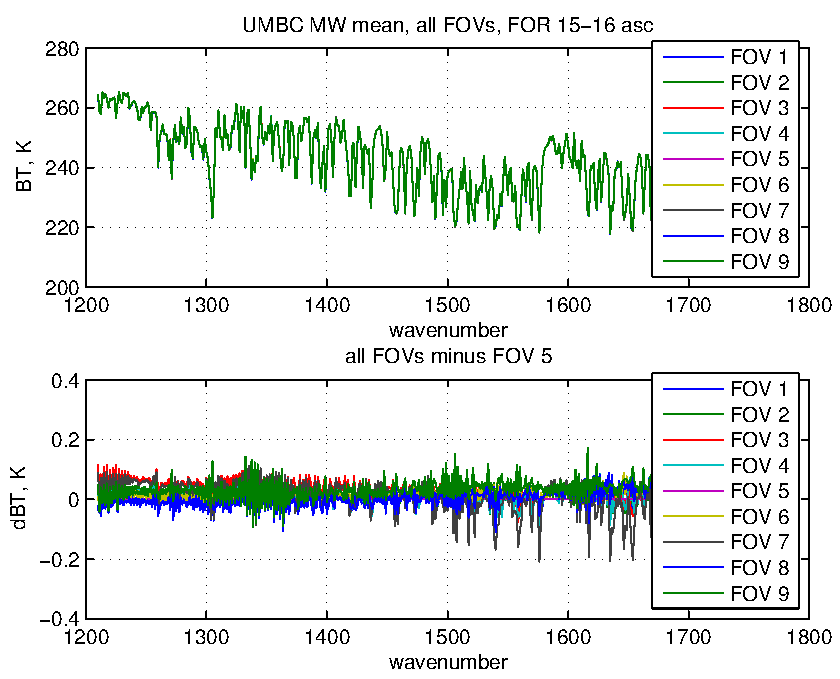
\includegraphics[scale=0.6]{umbc_MW_avg_5-18_Mar.pdf}
\end{center}

\ccast\ MW mean for all FOVs, and for all FOVs minus FOV 5

\end{frame}
%----------- slide --------------------------------------------------%
\begin{frame}
\frametitle{ccast MW 2-week test}

\begin{center}
  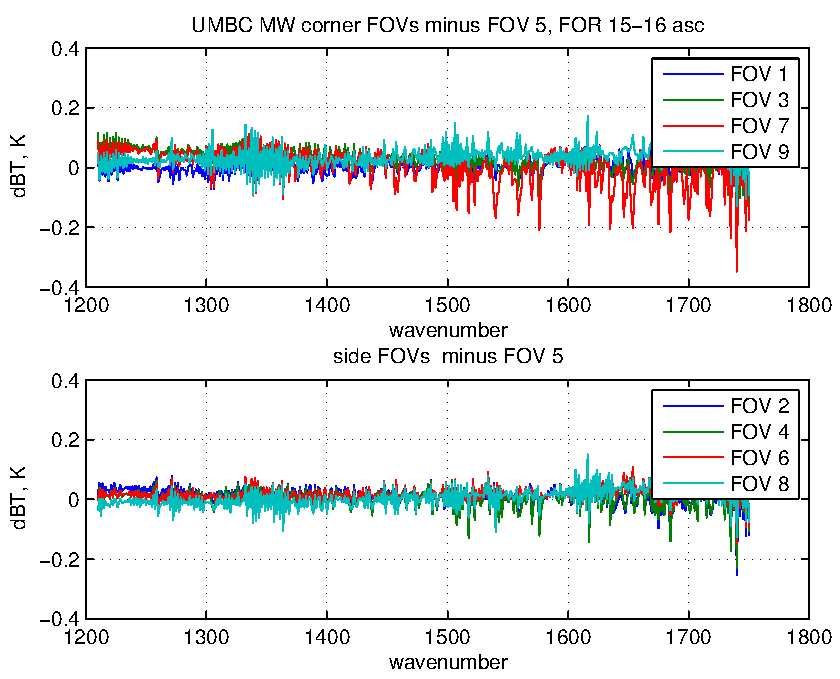
\includegraphics[scale=0.6]{umbc_MW_dif_5-18_Mar.pdf}
\end{center}

\ccast\ MW corner and side FOVs broken out separately

\end{frame}
%----------- slide --------------------------------------------------%
\begin{frame}
\frametitle{IDPS MW 2-week test}

\begin{center}
  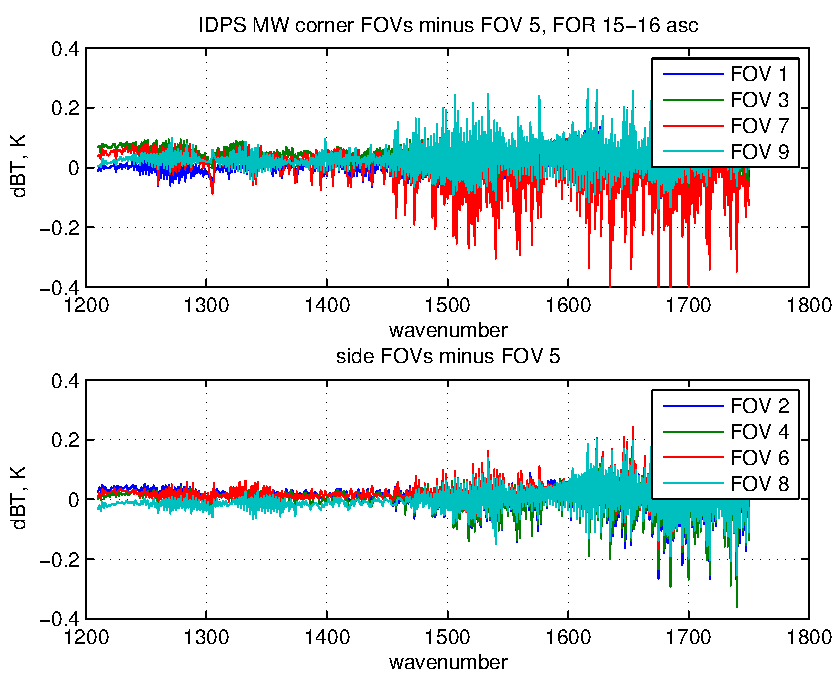
\includegraphics[scale=0.6]{idps_MW_dif_5-18_Mar.pdf}
\end{center}

\idps\ LW corner and side FOVs broken out separately

\end{frame}
%----------- slide --------------------------------------------------%
\begin{frame}
\frametitle{ccast MW 3-day $a_2$ test}

\begin{center}
  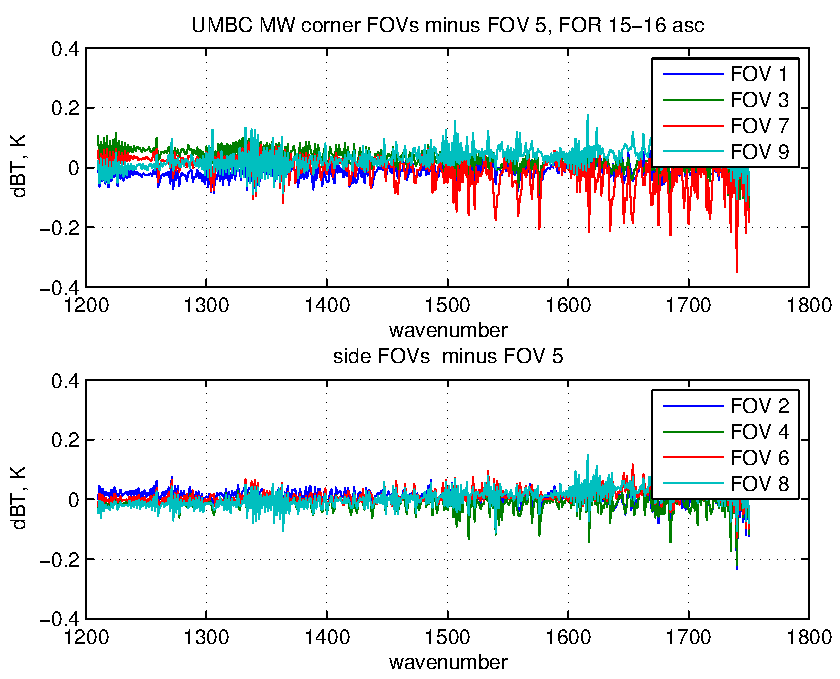
\includegraphics[scale=0.6]{umbc_MW_dif_1-3_Mar.pdf}
\end{center}

\ccast\ MW 3-day test with regular $a_2$ weights

\end{frame}
%----------- slide --------------------------------------------------%
\begin{frame}
\frametitle{ccast MW 3-day $a_2$ test}

\begin{center}
  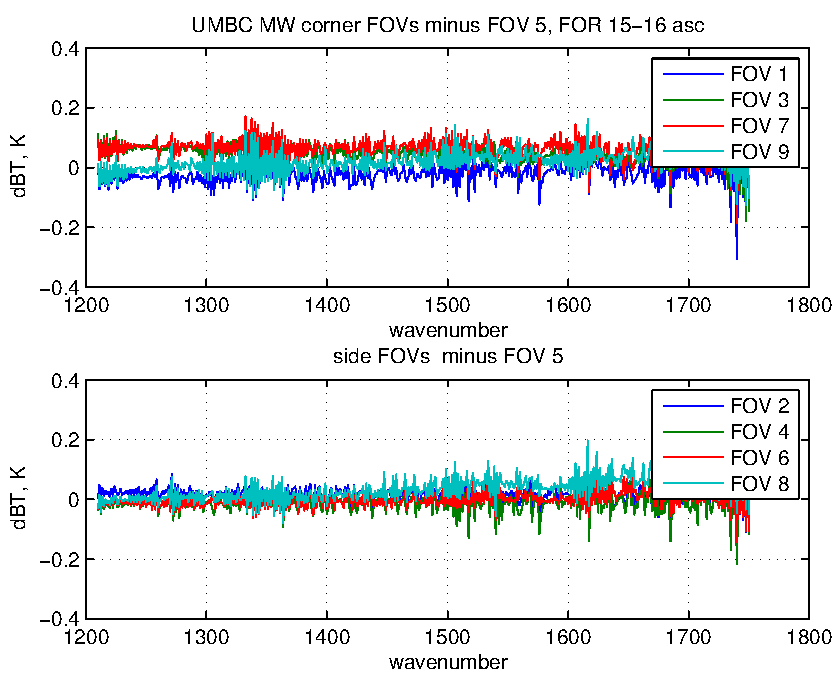
\includegraphics[scale=0.6]{umbc_MW_9a2_1-3_Mar.pdf}
\end{center}

\ccast\ MW test with $0.9 \cdot a_2$ weights.  FOVs 7 and 9 are
improved, especially FOV 7, while FOV 8 is a little worse

\end{frame}
%----------- slide --------------------------------------------------%
\begin{frame}
\frametitle{ccast high res test}

\begin{center}
  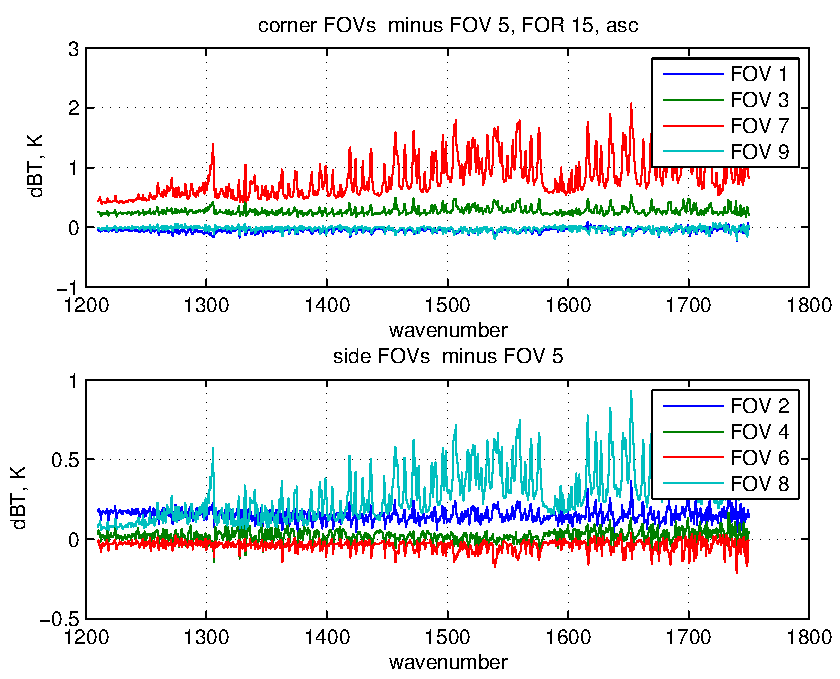
\includegraphics[scale=0.6]{hires_no_corr.pdf}
\end{center}

\ccast\ 27-28 Aug 2013 high res test with no nonlinearity
correction.  FOVs 7 and 8 are significantly out of group.

\end{frame}
%----------- slide --------------------------------------------------%
\begin{frame}
\frametitle{ccast high res test}

\begin{center}
  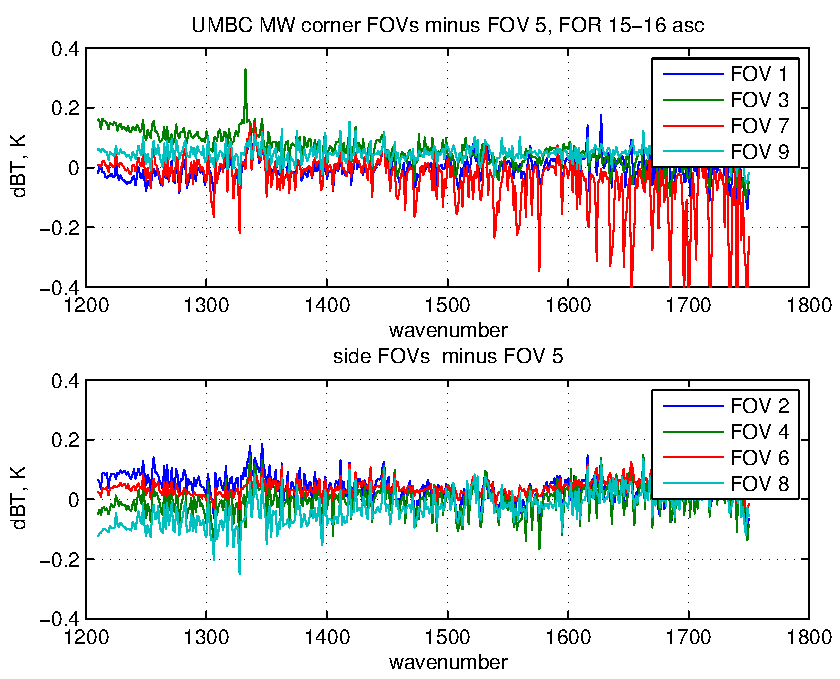
\includegraphics[scale=0.6]{hires_ref_corr.pdf}
\end{center}

\ccast\ 27-28 Aug 2013 high res test with regular $a_2$ weights

\end{frame}
%----------- slide --------------------------------------------------%
\begin{frame}
\frametitle{ccast high res test}

\begin{center}
  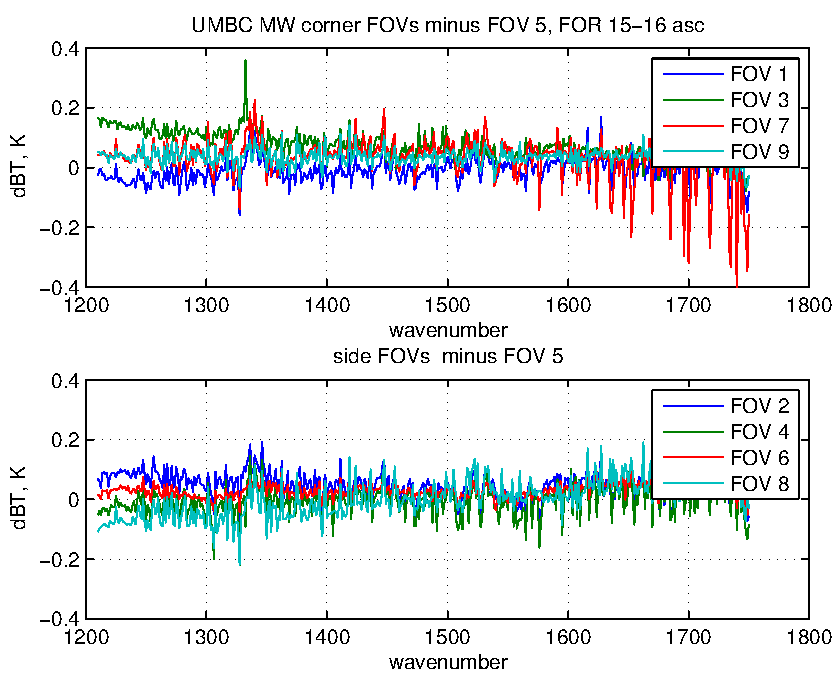
\includegraphics[scale=0.6]{hires_9a2_corr.pdf}
\end{center}

\ccast\ 27-28 Aug 2013 high res test with $0.9 \cdot a_2$ weights

\end{frame}
%----------- slide --------------------------------------------------%
\begin{frame}
\frametitle{1635 cm$^{-1}$ cold diffs}

\begin{center}
  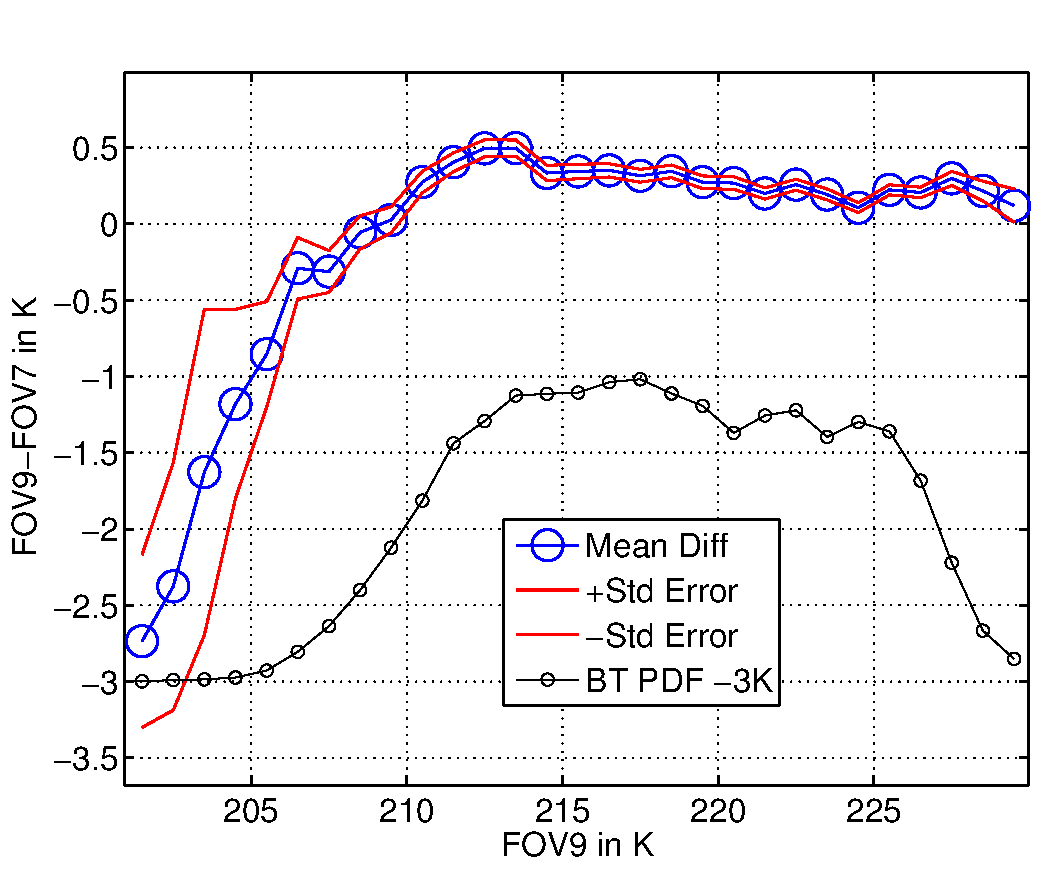
\includegraphics[scale=0.5]{strow/binned_chan1635wn_fov9_minus_fov7_versus_fov7.pdf}
\end{center}

1635 cm$^{-1}$ cold FOV 9 minus FOV 7 brightness temp diffs

\end{frame}
%----------- slide --------------------------------------------------%
\begin{frame}
\frametitle{1635 cm$^{-1}$ cold diffs}

\begin{center}
  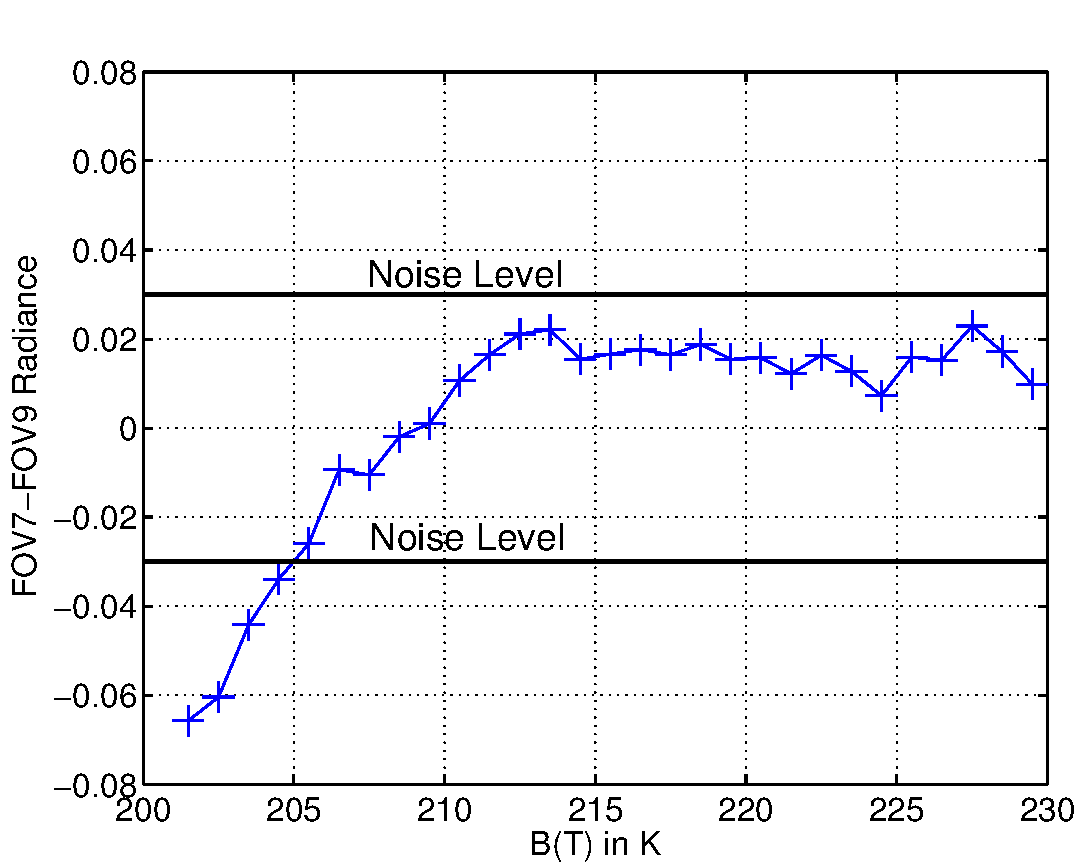
\includegraphics[scale=0.5]{strow/binned_chan1635wn_fov9_minus_fov7_radiance.pdf}
\end{center}

1635 cm$^{-1}$ cold FOV 7 minus FOV 9 radiance diffs

\end{frame}
%----------- slide --------------------------------------------------%
\begin{frame}
\frametitle{conclusions}

\begin{itemize}
  \item all tests were done without any added apodization

  \item our test for variation of FOV response, averaging and then
    comparing individual FOVs over relatively long time spans, seems
    to be valid

  \item these initial tests are comparisons with FOV 5 rather 
    than the most linear FOV to help sort out geometric or other
    variations in FOV response from nonlinearity

  \item MW FOVs 7 and 9 may need adjustment of the $a_2$ weights

  \item the large difference for MW FOV 7 may be due to problems 
    with cold scenes, or may require a second-order correction term

  \item the ccast nonlinearity correction works in high res mode

\end{itemize}

\end{frame}
%----------- slide --------------------------------------------------%
\end{document}

